% =============================================================================
% My Claude Code Workflow for Empirical Research
% A Visual Guide to AI-Assisted Research
% =============================================================================

\documentclass[aspectratio=169,11pt]{beamer}

% -----------------------------------------------------------------------------
% PACKAGES
% -----------------------------------------------------------------------------
\usepackage[utf8]{inputenc}
\usepackage[T1]{fontenc}
\usepackage{lmodern}
\usepackage{microtype}
\usepackage{amsmath,amssymb}
\usepackage{booktabs}
\usepackage{graphicx}
\usepackage{tikz}
\usepackage{pgfplots}
\usepackage{xcolor}
\usepackage{fontawesome5}
\usepackage{ragged2e}
\usepackage{colortbl}
\usepackage{array}
\usepackage{multirow}
\usepackage{hyperref}

\usetikzlibrary{shapes.geometric, arrows.meta, positioning, calc, backgrounds,
                decorations.pathreplacing, shadows, fadings, patterns}
\pgfplotsset{compat=1.18}

% -----------------------------------------------------------------------------
% COLOR PALETTE - Warm, energetic, professional
% -----------------------------------------------------------------------------
\definecolor{Midnight}{HTML}{1A1A2E}
\definecolor{DeepBlue}{HTML}{16213E}
\definecolor{RoyalBlue}{HTML}{0F3460}
\definecolor{Coral}{HTML}{E94560}
\definecolor{Sunset}{HTML}{F39C12}
\definecolor{Mint}{HTML}{1ABC9C}
\definecolor{Lavender}{HTML}{9B59B6}
\definecolor{SoftGray}{HTML}{BDC3C7}
\definecolor{LightGray}{HTML}{ECF0F1}
\definecolor{CloudWhite}{HTML}{FAFBFC}
\definecolor{Charcoal}{HTML}{2C3E50}
\definecolor{Success}{HTML}{27AE60}
\definecolor{Warning}{HTML}{E67E22}
\definecolor{Danger}{HTML}{C0392B}

% Set beamer colors
\setbeamercolor{normal text}{fg=Charcoal,bg=CloudWhite}
\setbeamercolor{structure}{fg=DeepBlue}
\setbeamercolor{alerted text}{fg=Coral}
\setbeamercolor{example text}{fg=Mint}

\setbeamercolor{palette primary}{bg=DeepBlue,fg=white}
\setbeamercolor{palette secondary}{bg=RoyalBlue,fg=white}
\setbeamercolor{palette tertiary}{bg=Coral,fg=white}

\setbeamercolor{frametitle}{fg=DeepBlue,bg=CloudWhite}
\setbeamercolor{title}{fg=white}
\setbeamercolor{subtitle}{fg=LightGray}
\setbeamercolor{author}{fg=LightGray}

\setbeamercolor{block title}{bg=DeepBlue,fg=white}
\setbeamercolor{block body}{bg=LightGray,fg=Charcoal}
\setbeamercolor{block title alerted}{bg=Coral,fg=white}
\setbeamercolor{block body alerted}{bg=LightGray,fg=Charcoal}
\setbeamercolor{block title example}{bg=Mint,fg=white}
\setbeamercolor{block body example}{bg=LightGray,fg=Charcoal}

% Item colors
\setbeamercolor{itemize item}{fg=Coral}
\setbeamercolor{itemize subitem}{fg=Mint}
\setbeamercolor{enumerate item}{fg=Coral}

% -----------------------------------------------------------------------------
% FONTS AND TYPOGRAPHY
% -----------------------------------------------------------------------------
\usefonttheme{professionalfonts}
\setbeamerfont{title}{size=\Huge,series=\bfseries}
\setbeamerfont{subtitle}{size=\large,series=\mdseries}
\setbeamerfont{frametitle}{size=\Large,series=\bfseries}
\setbeamerfont{framesubtitle}{size=\small,series=\mdseries}
\setbeamerfont{author}{size=\normalsize}
\setbeamerfont{footnote}{size=\tiny}

% -----------------------------------------------------------------------------
% BEAMER TEMPLATE CUSTOMIZATION
% -----------------------------------------------------------------------------
\setbeamertemplate{navigation symbols}{}
\setbeamertemplate{headline}{}

% Custom frame title
\setbeamertemplate{frametitle}{%
    \vspace{0.5cm}
    \begin{beamercolorbox}[wd=\paperwidth,leftskip=0.8cm]{frametitle}
        \usebeamerfont{frametitle}\insertframetitle
        \ifx\insertframesubtitle\empty\else
            \\[0.1cm]
            {\usebeamerfont{framesubtitle}\usebeamercolor[fg]{subtitle}\insertframesubtitle}
        \fi
    \end{beamercolorbox}
}

% Minimal footline with just page number
\setbeamertemplate{footline}{%
    \hfill
    \begin{beamercolorbox}[wd=3cm,ht=2.5ex,dp=1ex,right,rightskip=0.5cm]{page number}
        \usebeamercolor[fg]{SoftGray}\scriptsize\insertframenumber
    \end{beamercolorbox}
    \vspace{0.3cm}
}

% Itemize bullets
\setbeamertemplate{itemize item}{\footnotesize\raisebox{0.3ex}{\tikz\fill[Coral] (0,0) circle (0.5ex);}}
\setbeamertemplate{itemize subitem}{\footnotesize\raisebox{0.3ex}{\tikz\fill[Mint] (0,0) circle (0.4ex);}}

% Enumerate
\setbeamertemplate{enumerate item}{\textcolor{Coral}{\insertenumlabel.}}

% -----------------------------------------------------------------------------
% CUSTOM COMMANDS
% -----------------------------------------------------------------------------
\newcommand{\emphcoral}[1]{\textcolor{Coral}{\textbf{#1}}}
\newcommand{\emphmint}[1]{\textcolor{Mint}{\textbf{#1}}}
\newcommand{\emphsunset}[1]{\textcolor{Sunset}{\textbf{#1}}}
\newcommand{\graytext}[1]{\textcolor{SoftGray}{#1}}

% Transition slides
\newcommand{\transitionslide}[2]{%
    \begin{frame}[plain]
        \begin{tikzpicture}[remember picture,overlay]
            \fill[DeepBlue] (current page.south west) rectangle (current page.north east);
            % Decorative circles
            \fill[Coral,opacity=0.3] ([xshift=4cm,yshift=-2cm]current page.north west) circle (3cm);
            \fill[Mint,opacity=0.2] ([xshift=-3cm,yshift=3cm]current page.south east) circle (4cm);
            \node[anchor=center,text=white,font=\Huge\bfseries,text width=0.8\paperwidth,align=center]
                at ([yshift=0.5cm]current page.center) {#1};
            \node[anchor=center,text=LightGray,font=\large,text width=0.8\paperwidth,align=center,
                  below=1cm of current page.center] {#2};
        \end{tikzpicture}
    \end{frame}
}

% Key concept box
\newcommand{\conceptbox}[3]{%
    \begin{tikzpicture}
        \node[rectangle, rounded corners=8pt, fill=#1, text=white,
              minimum width=3.5cm, minimum height=1.2cm, font=\small\bfseries,
              align=center] (box) {#2};
        \node[below=0.2cm of box, text=Charcoal, font=\footnotesize,
              text width=3.5cm, align=center] {#3};
    \end{tikzpicture}
}

% -----------------------------------------------------------------------------
% DOCUMENT METADATA
% -----------------------------------------------------------------------------
\title{My Claude Code Workflow}
\subtitle{A Framework for AI-Assisted Empirical Research}
\author{Scott Cunningham}
\date{}

% =============================================================================
% DOCUMENT BEGINS
% =============================================================================
\begin{document}

% -----------------------------------------------------------------------------
% TITLE SLIDE
% -----------------------------------------------------------------------------
{
\setbeamertemplate{footline}{}
\begin{frame}[plain]
\begin{tikzpicture}[remember picture,overlay]
    % Gradient background
    \fill[DeepBlue] (current page.south west) rectangle (current page.north east);

    % Decorative elements
    \fill[Coral,opacity=0.4] ([xshift=-4cm,yshift=-4cm]current page.north east) circle (6cm);
    \fill[Mint,opacity=0.25] ([xshift=5cm,yshift=3cm]current page.south west) circle (5cm);
    \fill[Lavender,opacity=0.15] ([xshift=2cm,yshift=-1cm]current page.center) circle (3cm);

    % Grid pattern
    \foreach \i in {-6,-5,...,16} {
        \draw[white,opacity=0.03,line width=0.5pt]
            ([xshift=\i cm]current page.south west) -- ([xshift=\i cm]current page.north west);
    }
    \foreach \i in {-4,-3,...,10} {
        \draw[white,opacity=0.03,line width=0.5pt]
            ([yshift=\i cm]current page.south west) -- ([yshift=\i cm]current page.south east);
    }

    % Title
    \node[anchor=center,text=white,font=\fontsize{42}{46}\selectfont\bfseries,
          text width=0.85\paperwidth,align=center]
        at ([yshift=1.5cm]current page.center) {My Claude Code Workflow};

    % Subtitle
    \node[anchor=center,text=LightGray,font=\Large,
          text width=0.8\paperwidth,align=center]
        at ([yshift=-0.5cm]current page.center) {A Framework for AI-Assisted\\[0.2cm]Empirical Research};

    % Decorative line
    \draw[Coral,line width=3pt]
        ([yshift=-2cm,xshift=-4cm]current page.center) -- ([yshift=-2cm,xshift=4cm]current page.center);

    % Author
    \node[anchor=center,text=SoftGray,font=\normalsize]
        at ([yshift=-3cm]current page.center) {Scott Cunningham};
\end{tikzpicture}
\end{frame}
}

% -----------------------------------------------------------------------------
% THE CORE INSIGHT
% -----------------------------------------------------------------------------
\begin{frame}
\frametitle{The Core Insight}
\vspace{0.3cm}

\begin{center}
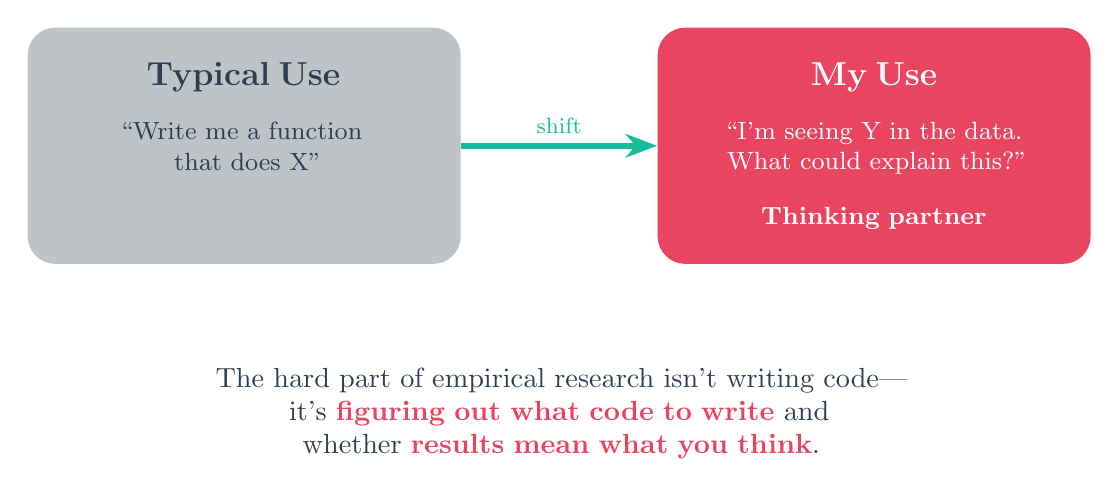
\begin{tikzpicture}
    % Two approaches side by side
    \node[rectangle, rounded corners=10pt, fill=SoftGray,
          minimum width=5.5cm, minimum height=3cm,
          text=Charcoal, font=\small, align=center, text width=5cm] (typical) at (-4,0) {
        \textbf{\large Typical Use}\\[0.3cm]
        ``Write me a function\\that does X''\\[0.3cm]
        \graytext{Code generator}
    };

    \node[rectangle, rounded corners=10pt, fill=Coral,
          minimum width=5.5cm, minimum height=3cm,
          text=white, font=\small, align=center, text width=5cm] (my) at (4,0) {
        \textbf{\large My Use}\\[0.3cm]
        ``I'm seeing Y in the data.\\What could explain this?''\\[0.3cm]
        \textbf{Thinking partner}
    };

    % Arrow
    \draw[-{Stealth[length=4mm,width=3mm]}, line width=2pt, Mint]
        (typical.east) -- (my.west) node[midway, above, font=\footnotesize, text=Mint] {shift};

    % Key message below
    \node[below=1.2cm of current bounding box.south, text=Charcoal,
          font=\normalsize, text width=11cm, align=center] {
        The hard part of empirical research isn't writing code---\\
        it's \emphcoral{figuring out what code to write} and whether \emphcoral{results mean what you think}.
    };
\end{tikzpicture}
\end{center}
\end{frame}

% -----------------------------------------------------------------------------
% THE FUNDAMENTAL PROBLEM
% -----------------------------------------------------------------------------
\begin{frame}
\frametitle{The Fundamental Problem: Claude Has Amnesia}
\vspace{0.3cm}

\begin{center}
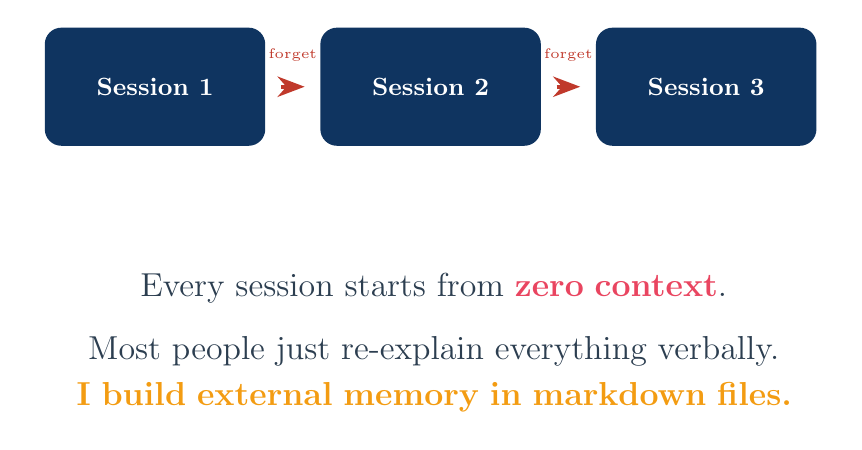
\begin{tikzpicture}
    % Session boxes
    \foreach \i/\label in {0/Session 1, 3.5/Session 2, 7/Session 3} {
        \node[rectangle, rounded corners=6pt, fill=RoyalBlue,
              minimum width=2.8cm, minimum height=1.5cm, text=white,
              font=\small\bfseries] at (\i, 0) {\label};
    }

    % Memory loss arrows
    \foreach \x in {1.6, 5.1} {
        \draw[-{Stealth}, line width=1.5pt, Danger, dashed]
            (\x, 0) -- (\x+0.3, 0);
        \node[above, font=\tiny, text=Danger] at (\x+0.15, 0.2) {forget};
    }

    % Brain icon (simplified)
    \node[below=1.5cm of current bounding box.south, text=Charcoal,
          font=\large, text width=10cm, align=center] {
        Every session starts from \emphcoral{zero context}.\\[0.3cm]
        Most people just re-explain everything verbally.\\[0.1cm]
        \emphsunset{I build external memory in markdown files.}
    };
\end{tikzpicture}
\end{center}
\end{frame}

% -----------------------------------------------------------------------------
% EXTERNAL MEMORY
% -----------------------------------------------------------------------------
\begin{frame}
\frametitle{External Memory via Markdown}
\vspace{0.2cm}

\begin{center}
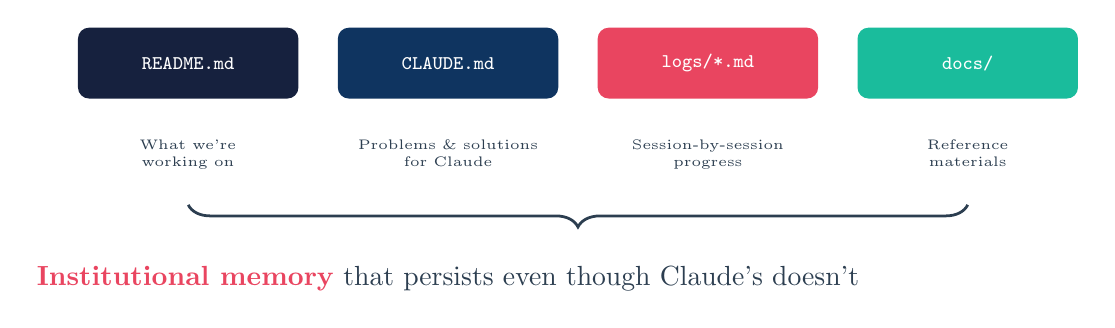
\begin{tikzpicture}[
    file/.style={rectangle, rounded corners=4pt, minimum width=2.8cm,
                 minimum height=0.9cm, font=\scriptsize\ttfamily,
                 text=white, align=center},
    desc/.style={font=\tiny, text=Charcoal, text width=2.8cm, align=center}
]
    % Files in a row
    \node[file, fill=DeepBlue] (readme) at (0,0) {README.md};
    \node[file, fill=RoyalBlue] (claude) at (3.3,0) {CLAUDE.md};
    \node[file, fill=Coral] (logs) at (6.6,0) {logs/*.md};
    \node[file, fill=Mint] (docs) at (9.9,0) {docs/};

    % Descriptions
    \node[desc, below=0.4cm of readme] {What we're\\working on};
    \node[desc, below=0.4cm of claude] {Problems \& solutions\\for Claude};
    \node[desc, below=0.4cm of logs] {Session-by-session\\progress};
    \node[desc, below=0.4cm of docs] {Reference\\materials};

    % Arrow pointing to central concept
    \draw[decorate, decoration={brace, amplitude=8pt, mirror}, line width=1pt, Charcoal]
        (0, -1.8) -- (9.9, -1.8);

    \node[below=0.8cm of claude, yshift=-1.2cm, text=Charcoal, font=\normalsize] {
        \emphcoral{Institutional memory} that persists even though Claude's doesn't
    };
\end{tikzpicture}
\end{center}
\end{frame}

% -----------------------------------------------------------------------------
% TRANSITION: THE PRACTICES
% -----------------------------------------------------------------------------
\transitionslide{Part I}{The Daily Practices}

% -----------------------------------------------------------------------------
% SOCRATIC METHOD
% -----------------------------------------------------------------------------
\begin{frame}
\frametitle{The Socratic Method for Alignment}
\vspace{0.1cm}

\begin{center}
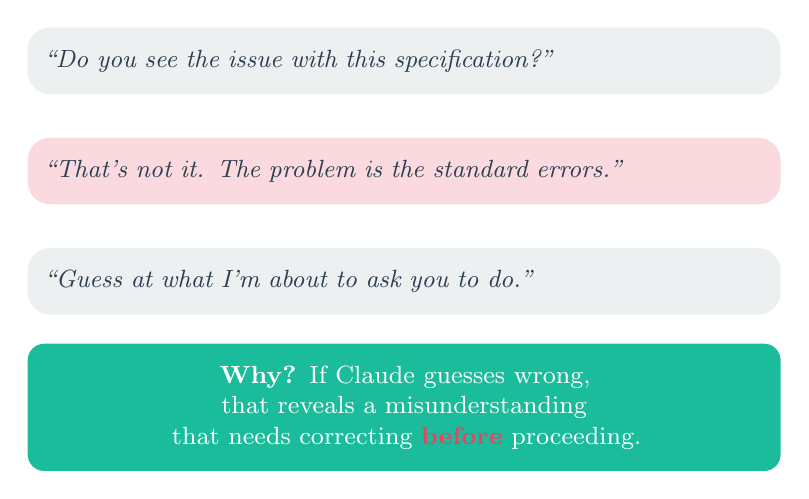
\begin{tikzpicture}
    % Conversation bubbles
    \node[rectangle, rounded corners=8pt, fill=LightGray,
          text width=9cm, font=\small, text=Charcoal,
          inner sep=8pt] (q1) at (0,1.8) {
        \textit{``Do you see the issue with this specification?''}
    };

    \node[rectangle, rounded corners=8pt, fill=Coral!20,
          text width=9cm, font=\small, text=Charcoal,
          inner sep=8pt] (q2) at (0,0.4) {
        \textit{``That's not it. The problem is the standard errors.''}
    };

    \node[rectangle, rounded corners=8pt, fill=LightGray,
          text width=9cm, font=\small, text=Charcoal,
          inner sep=8pt] (q3) at (0,-1) {
        \textit{``Guess at what I'm about to ask you to do.''}
    };

    % Why box
    \node[rectangle, rounded corners=6pt, fill=Mint, text=white,
          text width=9cm, font=\small, inner sep=8pt, align=center] at (0,-2.6) {
        \textbf{Why?} If Claude guesses wrong, that reveals a misunderstanding\\
        that needs correcting \emphcoral{before} proceeding.
    };
\end{tikzpicture}
\end{center}
\end{frame}

% -----------------------------------------------------------------------------
% SESSION STARTUP
% -----------------------------------------------------------------------------
\begin{frame}
\frametitle{Session Startup Routine}
\vspace{0.2cm}

\begin{center}
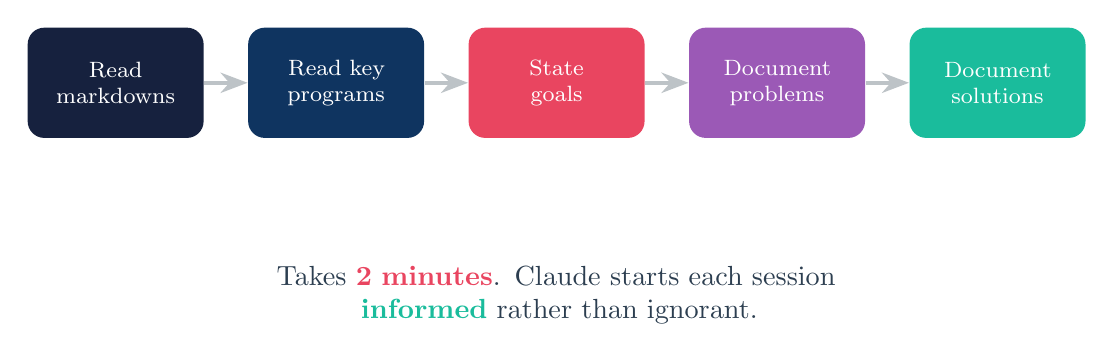
\begin{tikzpicture}
    % Steps in sequence
    \node[rectangle, rounded corners=6pt, fill=DeepBlue, text=white,
          minimum width=2.2cm, minimum height=1.4cm, font=\footnotesize,
          align=center, text width=2cm] (s1) at (0,0) {Read\\markdowns};
    \node[rectangle, rounded corners=6pt, fill=RoyalBlue, text=white,
          minimum width=2.2cm, minimum height=1.4cm, font=\footnotesize,
          align=center, text width=2cm] (s2) at (2.8,0) {Read key\\programs};
    \node[rectangle, rounded corners=6pt, fill=Coral, text=white,
          minimum width=2.2cm, minimum height=1.4cm, font=\footnotesize,
          align=center, text width=2cm] (s3) at (5.6,0) {State\\goals};
    \node[rectangle, rounded corners=6pt, fill=Lavender, text=white,
          minimum width=2.2cm, minimum height=1.4cm, font=\footnotesize,
          align=center, text width=2cm] (s4) at (8.4,0) {Document\\problems};
    \node[rectangle, rounded corners=6pt, fill=Mint, text=white,
          minimum width=2.2cm, minimum height=1.4cm, font=\footnotesize,
          align=center, text width=2cm] (s5) at (11.2,0) {Document\\solutions};

    % Arrows
    \draw[-{Stealth}, line width=1.5pt, SoftGray] (s1.east) -- (s2.west);
    \draw[-{Stealth}, line width=1.5pt, SoftGray] (s2.east) -- (s3.west);
    \draw[-{Stealth}, line width=1.5pt, SoftGray] (s3.east) -- (s4.west);
    \draw[-{Stealth}, line width=1.5pt, SoftGray] (s4.east) -- (s5.west);

    % Time note
    \node[below=1.5cm of s3, text=Charcoal, font=\normalsize, text width=10cm, align=center] {
        Takes \emphcoral{2 minutes}. Claude starts each session\\
        \emphmint{informed} rather than ignorant.
    };
\end{tikzpicture}
\end{center}
\end{frame}

% -----------------------------------------------------------------------------
% VERIFICATION THROUGH VISUALIZATION
% -----------------------------------------------------------------------------
\begin{frame}
\frametitle{Verification Through Visualization}
\vspace{0.3cm}

\begin{center}
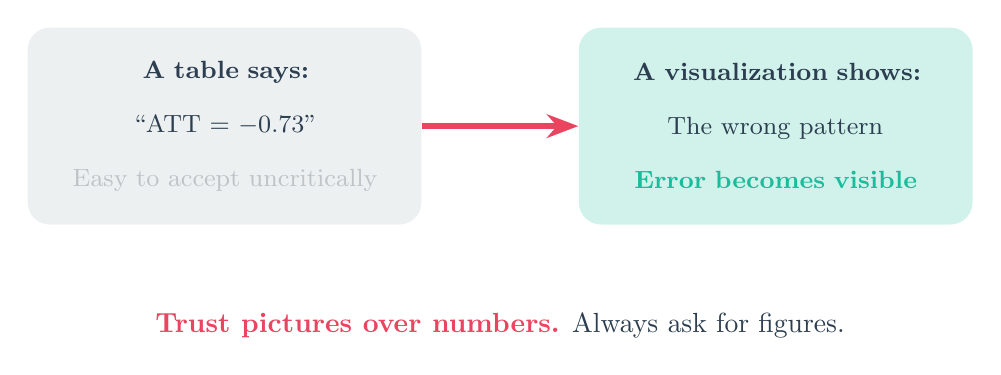
\begin{tikzpicture}
    % Two comparison boxes
    \node[rectangle, rounded corners=8pt, fill=LightGray,
          minimum width=5cm, minimum height=2.5cm,
          text=Charcoal, font=\small, align=center, text width=4.5cm] (table) at (-3.5,0) {
        \textbf{A table says:}\\[0.3cm]
        ``ATT = $-0.73$''\\[0.3cm]
        \graytext{Easy to accept uncritically}
    };

    \node[rectangle, rounded corners=8pt, fill=Mint!20,
          minimum width=5cm, minimum height=2.5cm,
          text=Charcoal, font=\small, align=center, text width=4.5cm] (viz) at (3.5,0) {
        \textbf{A visualization shows:}\\[0.3cm]
        The wrong pattern\\[0.3cm]
        \emphmint{Error becomes visible}
    };

    % Arrow
    \draw[-{Stealth[length=4mm,width=3mm]}, line width=2pt, Coral]
        (table.east) -- (viz.west);

    % Key message
    \node[below=1cm of current bounding box.south, text=Charcoal, font=\normalsize] {
        \emphcoral{Trust pictures over numbers.} Always ask for figures.
    };
\end{tikzpicture}
\end{center}
\end{frame}

% -----------------------------------------------------------------------------
% TRANSITION: CROSS-SOFTWARE
% -----------------------------------------------------------------------------
\transitionslide{Part II}{Cross-Software Replication}

% -----------------------------------------------------------------------------
% THE CORE INSIGHT OF CROSS-SOFTWARE
% -----------------------------------------------------------------------------
\begin{frame}
\frametitle{Bugs Are Orthogonal Across Languages}
\vspace{0.2cm}

\begin{center}
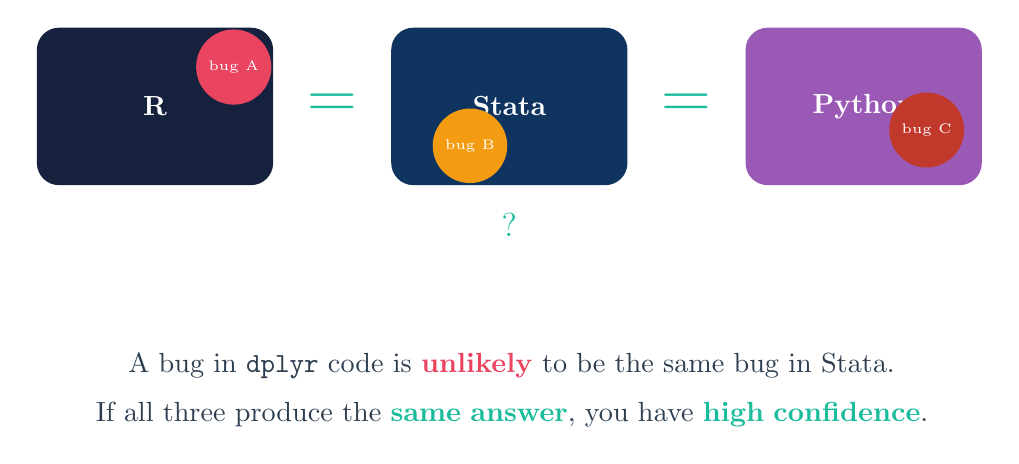
\begin{tikzpicture}
    % Three language boxes
    \node[rectangle, rounded corners=8pt, fill=DeepBlue,
          minimum width=3cm, minimum height=2cm, text=white,
          font=\bfseries] (r) at (0,0) {R};
    \node[rectangle, rounded corners=8pt, fill=RoyalBlue,
          minimum width=3cm, minimum height=2cm, text=white,
          font=\bfseries] (stata) at (4.5,0) {Stata};
    \node[rectangle, rounded corners=8pt, fill=Lavender,
          minimum width=3cm, minimum height=2cm, text=white,
          font=\bfseries] (python) at (9,0) {Python};

    % Bug indicators (different bugs)
    \node[circle, fill=Coral, minimum size=0.6cm, font=\tiny, text=white]
        at ([xshift=1cm,yshift=0.5cm]r.center) {bug A};
    \node[circle, fill=Sunset, minimum size=0.6cm, font=\tiny, text=white]
        at ([xshift=-0.5cm,yshift=-0.5cm]stata.center) {bug B};
    \node[circle, fill=Danger, minimum size=0.6cm, font=\tiny, text=white]
        at ([xshift=0.8cm,yshift=-0.3cm]python.center) {bug C};

    % Equals signs with question
    \node[font=\Huge, text=Mint] at (2.25, 0) {=};
    \node[font=\Huge, text=Mint] at (6.75, 0) {=};
    \node[font=\large, text=Mint] at (4.5, -1.5) {?};

    % Key insight
    \node[below=2cm of stata, text=Charcoal, font=\normalsize, text width=12cm, align=center] {
        A bug in \texttt{dplyr} code is \emphcoral{unlikely} to be the same bug in Stata.\\[0.2cm]
        If all three produce the \emphmint{same answer}, you have \emphmint{high confidence}.
    };
\end{tikzpicture}
\end{center}
\end{frame}

% -----------------------------------------------------------------------------
% WHY THIS WORKS
% -----------------------------------------------------------------------------
\begin{frame}
\frametitle{Why Cross-Language Validation Works}
\vspace{0.3cm}

\begin{center}
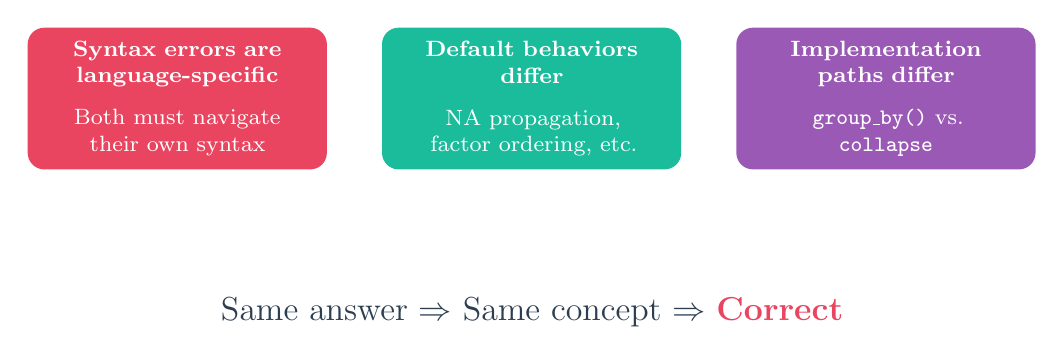
\begin{tikzpicture}
    % Three reasons
    \node[rectangle, rounded corners=6pt, fill=Coral, text=white,
          minimum width=3.8cm, minimum height=1.8cm, font=\footnotesize,
          align=center, text width=3.5cm] (r1) at (0,0) {\textbf{Syntax errors are}\\
        \textbf{language-specific}\\[0.2cm]
        Both must navigate\\their own syntax};

    \node[rectangle, rounded corners=6pt, fill=Mint, text=white,
          minimum width=3.8cm, minimum height=1.8cm, font=\footnotesize,
          align=center, text width=3.5cm] (r2) at (4.5,0) {\textbf{Default behaviors}\\
        \textbf{differ}\\[0.2cm]
        NA propagation,\\factor ordering, etc.};

    \node[rectangle, rounded corners=6pt, fill=Lavender, text=white,
          minimum width=3.8cm, minimum height=1.8cm, font=\footnotesize,
          align=center, text width=3.5cm] (r3) at (9,0) {\textbf{Implementation}\\
        \textbf{paths differ}\\[0.2cm]
        \texttt{group\_by()} vs.\\
        \texttt{collapse}};

    % Bottom message
    \node[below=1.5cm of r2, text=Charcoal, font=\large, text width=10cm, align=center] {
        Same answer $\Rightarrow$ Same concept $\Rightarrow$ \emphcoral{Correct}
    };
\end{tikzpicture}
\end{center}
\end{frame}

% -----------------------------------------------------------------------------
% THE COMPARISON TABLE
% -----------------------------------------------------------------------------
\begin{frame}
\frametitle{The Validation Table}
\vspace{0.2cm}

\begin{center}
\begin{tikzpicture}
    % Table
    \node[inner sep=0pt] at (0,0) {
        \begin{tabular}{lccc}
            \toprule
            \textbf{Check} & \textbf{R} & \textbf{Stata} & \textbf{Match?} \\
            \midrule
            Sample rows & 5,234 & 5,234 & \textcolor{Success}{\faCheck} \\
            Mean age (treatment) & 31.7 & 31.7 & \textcolor{Success}{\faCheck} \\
            Mean hourly wage & \$5.43 & \$5.43 & \textcolor{Success}{\faCheck} \\
            N missing earnings & 412 & 412 & \textcolor{Success}{\faCheck} \\
            \bottomrule
        \end{tabular}
    };

    % Note below
    \node[below=1.5cm of current bounding box.south, text=Charcoal,
          font=\normalsize, text width=10cm, align=center] {
        If any differ $\Rightarrow$ \emphcoral{investigate before proceeding}.\\[0.2cm]
        This isn't paranoia. It's \emphmint{methodology}.
    };
\end{tikzpicture}
\end{center}
\end{frame}

% -----------------------------------------------------------------------------
% TRANSITION: REFEREE 2
% -----------------------------------------------------------------------------
\transitionslide{Part III}{Adversarial Review}

% -----------------------------------------------------------------------------
% THE PROBLEM WITH SELF-REVIEW
% -----------------------------------------------------------------------------
\begin{frame}
\frametitle{You Can't Grade Your Own Homework}
\vspace{0.3cm}

\begin{center}
\begin{tikzpicture}
    % Same Claude reviewing its own work
    \node[rectangle, rounded corners=10pt, fill=LightGray,
          minimum width=4cm, minimum height=2.5cm,
          text=Charcoal, align=center, text width=3.5cm] (claude1) at (-3,0) {
        \textbf{Claude writes code}\\[0.3cm]
        (makes subtle choices,\\
        cuts corners)
    };

    \node[rectangle, rounded corners=10pt, fill=LightGray,
          minimum width=4cm, minimum height=2.5cm,
          text=Charcoal, align=center, text width=3.5cm] (claude2) at (3,0) {
        \textbf{Same Claude reviews}\\[0.3cm]
        (rationalizes choices,\\
        misses problems)
    };

    % Arrow with X
    \draw[-{Stealth}, line width=2pt, Danger] (claude1.east) -- (claude2.west);
    \node[circle, fill=Danger, text=white, font=\bfseries] at (0,0.5) {\faTimes};

    % Problem statement
    \node[rectangle, rounded corners=6pt, fill=Coral, text=white,
          font=\normalsize, inner sep=10pt, text width=10cm, align=center]
        at (0,-2.5) {
        Asking the same Claude to review its own code is like\\
        asking a student to grade their own exam.
    };
\end{tikzpicture}
\end{center}
\end{frame}

% -----------------------------------------------------------------------------
% THE SOLUTION: REFEREE 2
% -----------------------------------------------------------------------------
\begin{frame}
\frametitle{The Solution: Referee 2 Protocol}
\vspace{0.2cm}

\begin{center}
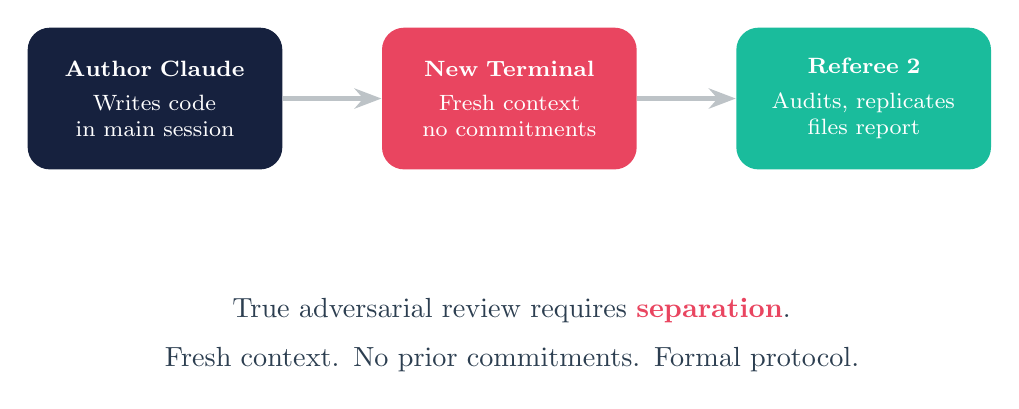
\begin{tikzpicture}
    % Flow
    \node[rectangle, rounded corners=8pt, fill=DeepBlue, text=white,
          minimum width=3.2cm, minimum height=1.8cm, font=\footnotesize,
          align=center, text width=3cm] (author) at (0,0) {\textbf{Author Claude}\\[0.1cm]
        Writes code\\in main session};

    \node[rectangle, rounded corners=8pt, fill=Coral, text=white,
          minimum width=3.2cm, minimum height=1.8cm, font=\footnotesize,
          align=center, text width=3cm] (new) at (4.5,0) {\textbf{New Terminal}\\[0.1cm]
        Fresh context\\no commitments};

    \node[rectangle, rounded corners=8pt, fill=Mint, text=white,
          minimum width=3.2cm, minimum height=1.8cm, font=\footnotesize,
          align=center, text width=3cm] (ref2) at (9,0) {\textbf{Referee 2}\\[0.1cm]
        Audits, replicates\\files report};

    % Arrows
    \draw[-{Stealth}, line width=1.5pt, SoftGray] (author.east) -- (new.west);
    \draw[-{Stealth}, line width=1.5pt, SoftGray] (new.east) -- (ref2.west);

    % Key point
    \node[below=1.5cm of new, text=Charcoal, font=\normalsize, text width=10cm, align=center] {
        True adversarial review requires \emphcoral{separation}.\\[0.2cm]
        Fresh context. No prior commitments. Formal protocol.
    };
\end{tikzpicture}
\end{center}
\end{frame}

% -----------------------------------------------------------------------------
% THE FIVE AUDITS
% -----------------------------------------------------------------------------
\begin{frame}
\frametitle{The Five Audits}
\vspace{0.1cm}

\begin{center}
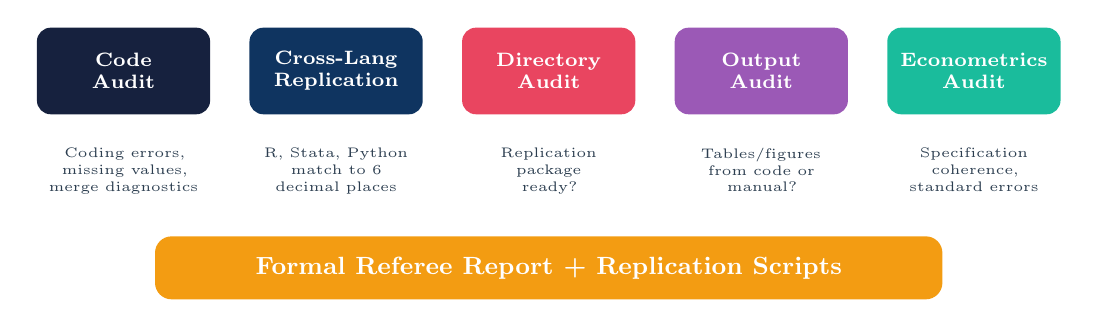
\begin{tikzpicture}
    % Five audits
    \node[rectangle, rounded corners=5pt, fill=DeepBlue, text=white,
          minimum width=2.2cm, minimum height=1.1cm, font=\scriptsize\bfseries,
          align=center] (a1) at (0,0) {Code\\Audit};
    \node[rectangle, rounded corners=5pt, fill=RoyalBlue, text=white,
          minimum width=2.2cm, minimum height=1.1cm, font=\scriptsize\bfseries,
          align=center] (a2) at (2.7,0) {Cross-Lang\\Replication};
    \node[rectangle, rounded corners=5pt, fill=Coral, text=white,
          minimum width=2.2cm, minimum height=1.1cm, font=\scriptsize\bfseries,
          align=center] (a3) at (5.4,0) {Directory\\Audit};
    \node[rectangle, rounded corners=5pt, fill=Lavender, text=white,
          minimum width=2.2cm, minimum height=1.1cm, font=\scriptsize\bfseries,
          align=center] (a4) at (8.1,0) {Output\\Audit};
    \node[rectangle, rounded corners=5pt, fill=Mint, text=white,
          minimum width=2.2cm, minimum height=1.1cm, font=\scriptsize\bfseries,
          align=center] (a5) at (10.8,0) {Econometrics\\Audit};

    % Descriptions
    \node[font=\tiny, text=Charcoal, text width=2.2cm, align=center, below=0.3cm of a1] {Coding errors,\\missing values,\\merge diagnostics};
    \node[font=\tiny, text=Charcoal, text width=2.2cm, align=center, below=0.3cm of a2] {R, Stata, Python\\match to 6\\decimal places};
    \node[font=\tiny, text=Charcoal, text width=2.2cm, align=center, below=0.3cm of a3] {Replication\\package\\ready?};
    \node[font=\tiny, text=Charcoal, text width=2.2cm, align=center, below=0.3cm of a4] {Tables/figures\\from code or\\manual?};
    \node[font=\tiny, text=Charcoal, text width=2.2cm, align=center, below=0.3cm of a5] {Specification\\coherence,\\standard errors};

    % Output
    \node[rectangle, rounded corners=6pt, fill=Sunset, text=white,
          minimum width=10cm, minimum height=0.8cm, font=\small\bfseries]
        at (5.4,-2.5) {Formal Referee Report + Replication Scripts};
\end{tikzpicture}
\end{center}
\end{frame}

% -----------------------------------------------------------------------------
% WHAT REFEREE 2 CATCHES
% -----------------------------------------------------------------------------
\begin{frame}
\frametitle{What Referee 2 Catches}
\vspace{0.3cm}

\begin{center}
\begin{tikzpicture}
    % List of catches
    \node[rectangle, rounded corners=4pt, fill=LightGray,
          text=Charcoal, minimum height=0.8cm, font=\small,
          inner xsep=12pt, inner ysep=6pt] (c1) at (0,2) {\textbf{Unstated assumptions} --- ``Did you verify X or just assume it?''};
    \node[rectangle, rounded corners=4pt, fill=LightGray,
          text=Charcoal, minimum height=0.8cm, font=\small,
          inner xsep=12pt, inner ysep=6pt] (c2) at (0,1) {\textbf{Alternative explanations} --- ``Could the pattern come from something else?''};
    \node[rectangle, rounded corners=4pt, fill=LightGray,
          text=Charcoal, minimum height=0.8cm, font=\small,
          inner xsep=12pt, inner ysep=6pt] (c3) at (0,0) {\textbf{Documentation gaps} --- ``Where does it explicitly say this?''};
    \node[rectangle, rounded corners=4pt, fill=LightGray,
          text=Charcoal, minimum height=0.8cm, font=\small,
          inner xsep=12pt, inner ysep=6pt] (c4) at (0,-1) {\textbf{Logical leaps} --- ``You concluded A, but evidence only supports B''};
    \node[rectangle, rounded corners=4pt, fill=LightGray,
          text=Charcoal, minimum height=0.8cm, font=\small,
          inner xsep=12pt, inner ysep=6pt] (c5) at (0,-2) {\textbf{Missing verification} --- ``Have you actually checked the raw data?''};

    % Check marks
    \node[left=0.3cm of c1, text=Mint, font=\large] {\faCheck};
    \node[left=0.3cm of c2, text=Mint, font=\large] {\faCheck};
    \node[left=0.3cm of c3, text=Mint, font=\large] {\faCheck};
    \node[left=0.3cm of c4, text=Mint, font=\large] {\faCheck};
    \node[left=0.3cm of c5, text=Mint, font=\large] {\faCheck};
\end{tikzpicture}
\end{center}
\end{frame}

% -----------------------------------------------------------------------------
% THE PHILOSOPHY
% -----------------------------------------------------------------------------
\begin{frame}
\frametitle{The Philosophy}
\vspace{0.3cm}

\begin{center}
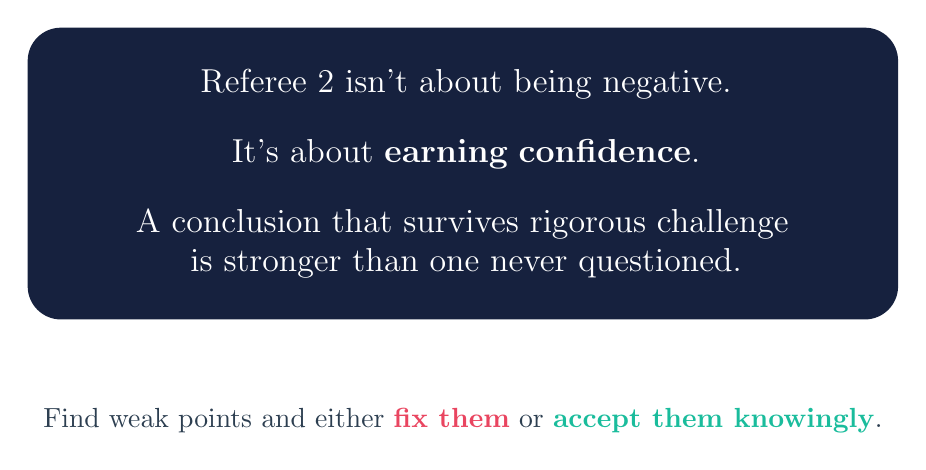
\begin{tikzpicture}
    \node[rectangle, rounded corners=12pt, fill=DeepBlue, text=white,
          minimum width=11cm, minimum height=3cm, font=\large,
          align=center, text width=10cm, inner sep=15pt] {
        Referee 2 isn't about being negative.\\[0.4cm]
        It's about \textbf{earning confidence}.\\[0.4cm]
        A conclusion that survives rigorous challenge\\
        is stronger than one never questioned.
    };

    \node[below=1cm of current bounding box.south, text=Charcoal, font=\normalsize] {
        Find weak points and either \emphcoral{fix them} or \emphmint{accept them knowingly}.
    };
\end{tikzpicture}
\end{center}
\end{frame}

% -----------------------------------------------------------------------------
% TRANSITION: WHY THIS WORKS
% -----------------------------------------------------------------------------
\transitionslide{Part IV}{Why This Works}

% -----------------------------------------------------------------------------
% PRODUCT VS RESEARCH
% -----------------------------------------------------------------------------
\begin{frame}
\frametitle{Research Is Not Product Development}
\vspace{0.2cm}

\begin{center}
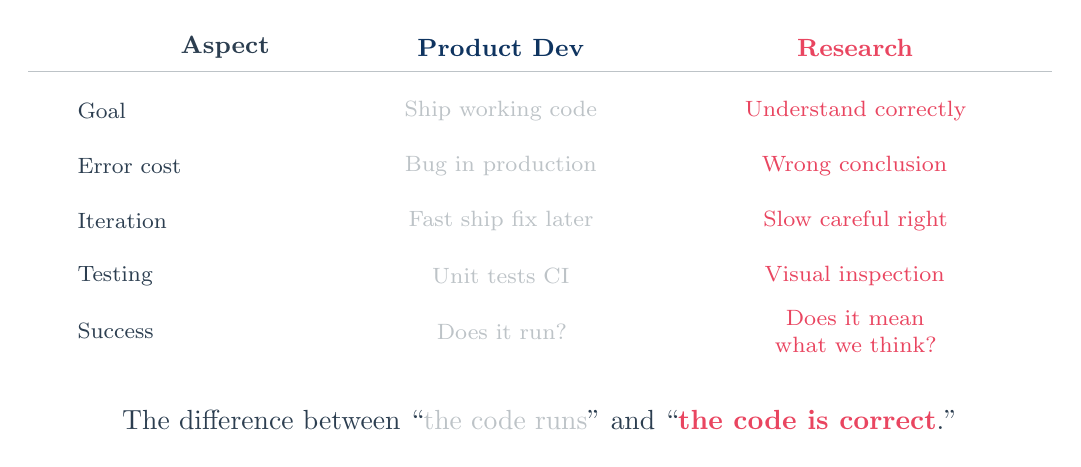
\begin{tikzpicture}
    % Headers
    \node[font=\small\bfseries, text=Charcoal] at (-4, 2.2) {Aspect};
    \node[font=\small\bfseries, text=RoyalBlue] at (-0.5, 2.2) {Product Dev};
    \node[font=\small\bfseries, text=Coral] at (4, 2.2) {Research};

    % Divider
    \draw[SoftGray, line width=0.5pt] (-6.5, 1.9) -- (6.5, 1.9);

    % Rows - expanded manually
    \node[font=\footnotesize, text=Charcoal, anchor=west] at (-6, 1.4) {Goal};
    \node[font=\footnotesize, text=SoftGray, text width=3cm, align=center] at (-0.5, 1.4) {Ship working code};
    \node[font=\footnotesize, text=Coral, text width=3.5cm, align=center] at (4, 1.4) {Understand correctly};

    \node[font=\footnotesize, text=Charcoal, anchor=west] at (-6, 0.7) {Error cost};
    \node[font=\footnotesize, text=SoftGray, text width=3cm, align=center] at (-0.5, 0.7) {Bug in production};
    \node[font=\footnotesize, text=Coral, text width=3.5cm, align=center] at (4, 0.7) {Wrong conclusion};

    \node[font=\footnotesize, text=Charcoal, anchor=west] at (-6, 0) {Iteration};
    \node[font=\footnotesize, text=SoftGray, text width=3cm, align=center] at (-0.5, 0) {Fast ship fix later};
    \node[font=\footnotesize, text=Coral, text width=3.5cm, align=center] at (4, 0) {Slow careful right};

    \node[font=\footnotesize, text=Charcoal, anchor=west] at (-6, -0.7) {Testing};
    \node[font=\footnotesize, text=SoftGray, text width=3cm, align=center] at (-0.5, -0.7) {Unit tests CI};
    \node[font=\footnotesize, text=Coral, text width=3.5cm, align=center] at (4, -0.7) {Visual inspection};

    \node[font=\footnotesize, text=Charcoal, anchor=west] at (-6, -1.4) {Success};
    \node[font=\footnotesize, text=SoftGray, text width=3cm, align=center] at (-0.5, -1.4) {Does it run?};
    \node[font=\footnotesize, text=Coral, text width=3.5cm, align=center] at (4, -1.4) {Does it mean what we think?};

    % Bottom insight
    \node[below=0.5cm of current bounding box.south, text=Charcoal, font=\normalsize] {
        The difference between ``\graytext{the code runs}'' and ``\emphcoral{the code is correct}.''
    };
\end{tikzpicture}
\end{center}
\end{frame}

% -----------------------------------------------------------------------------
% THE STAKES
% -----------------------------------------------------------------------------
\begin{frame}
\frametitle{The Stakes Are Different}
\vspace{0.3cm}

\begin{center}
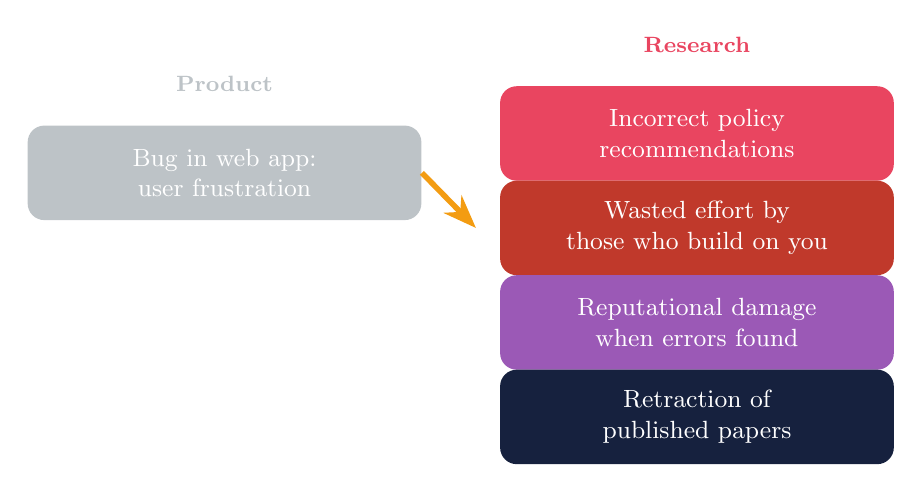
\begin{tikzpicture}
    % Stakes
    \node[rectangle, rounded corners=6pt, fill=SoftGray, text=white,
          minimum width=5cm, minimum height=1.2cm, font=\small,
          align=center] (s1) at (-3,1.5) {Bug in web app:\\user frustration};

    \node[rectangle, rounded corners=6pt, fill=Coral, text=white,
          minimum width=5cm, minimum height=1.2cm, font=\small,
          align=center] (s2) at (3,2) {Incorrect policy\\recommendations};
    \node[rectangle, rounded corners=6pt, fill=Danger, text=white,
          minimum width=5cm, minimum height=1.2cm, font=\small,
          align=center] (s3) at (3,0.8) {Wasted effort by\\those who build on you};
    \node[rectangle, rounded corners=6pt, fill=Lavender, text=white,
          minimum width=5cm, minimum height=1.2cm, font=\small,
          align=center] (s4) at (3,-0.4) {Reputational damage\\when errors found};
    \node[rectangle, rounded corners=6pt, fill=DeepBlue, text=white,
          minimum width=5cm, minimum height=1.2cm, font=\small,
          align=center] (s5) at (3,-1.6) {Retraction of\\published papers};

    % Arrow
    \draw[-{Stealth}, line width=2pt, Sunset] (s1.east) -- ([xshift=-0.3cm]s3.west);

    % Labels
    \node[above=0.3cm of s1, font=\footnotesize\bfseries, text=SoftGray] {Product};
    \node[above=0.3cm of s2, font=\footnotesize\bfseries, text=Coral] {Research};
\end{tikzpicture}
\end{center}
\end{frame}

% -----------------------------------------------------------------------------
% SUMMARY TABLE
% -----------------------------------------------------------------------------
\begin{frame}
\frametitle{The Workflow in Summary}
\vspace{0.2cm}

\begin{center}
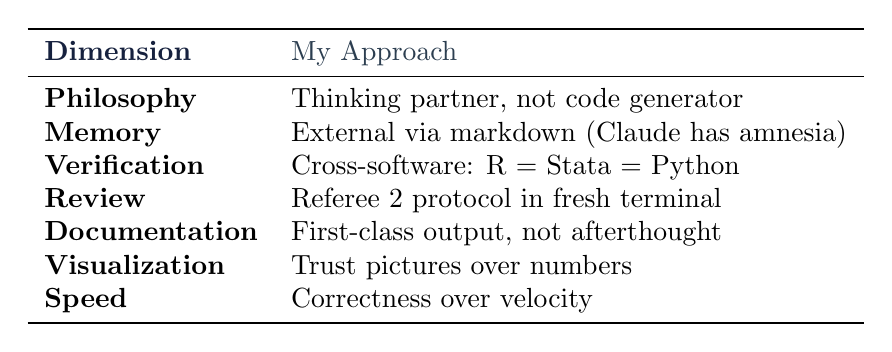
\begin{tikzpicture}
    \node[inner sep=0pt] {
        \begin{tabular}{>{\bfseries}l l}
            \toprule
            \textcolor{DeepBlue}{Dimension} & \textcolor{Charcoal}{My Approach} \\
            \midrule
            Philosophy & Thinking partner, not code generator \\
            Memory & External via markdown (Claude has amnesia) \\
            Verification & Cross-software: R = Stata = Python \\
            Review & Referee 2 protocol in fresh terminal \\
            Documentation & First-class output, not afterthought \\
            Visualization & Trust pictures over numbers \\
            Speed & Correctness over velocity \\
            \bottomrule
        \end{tabular}
    };
\end{tikzpicture}
\end{center}
\end{frame}

% -----------------------------------------------------------------------------
% THE KEY INSIGHT
% -----------------------------------------------------------------------------
\begin{frame}
\frametitle{The Key Insight}
\vspace{0.5cm}

\begin{center}
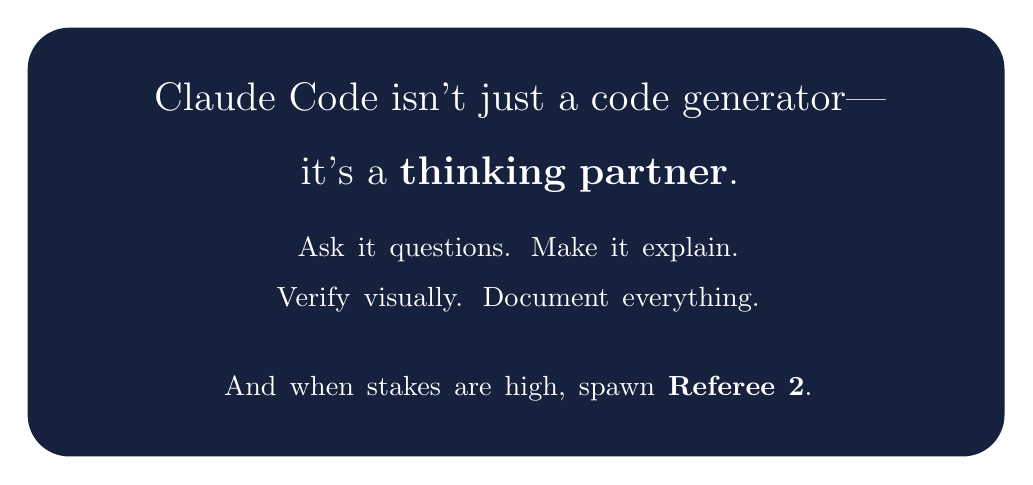
\begin{tikzpicture}
    \node[rectangle, rounded corners=15pt, fill=DeepBlue, text=white,
          minimum width=12cm, minimum height=4cm, font=\Large,
          align=center, text width=11cm, inner sep=20pt] {
        Claude Code isn't just a code generator---\\[0.3cm]
        it's a \textbf{thinking partner}.\\[0.5cm]
        {\normalsize Ask it questions. Make it explain.\\
        Verify visually. Document everything.}\\[0.5cm]
        {\normalsize And when stakes are high, spawn \textbf{Referee 2}.}
    };
\end{tikzpicture}
\end{center}
\end{frame}

% -----------------------------------------------------------------------------
% CLOSING
% -----------------------------------------------------------------------------
{
\setbeamertemplate{footline}{}
\begin{frame}[plain]
\begin{tikzpicture}[remember picture,overlay]
    % Background
    \fill[DeepBlue] (current page.south west) rectangle (current page.north east);

    % Decorative elements
    \fill[Coral,opacity=0.3] ([xshift=-3cm,yshift=-3cm]current page.north east) circle (5cm);
    \fill[Mint,opacity=0.2] ([xshift=4cm,yshift=2cm]current page.south west) circle (4cm);

    % Title
    \node[anchor=center,text=white,font=\Huge\bfseries,
          text width=0.8\paperwidth,align=center]
        at ([yshift=1cm]current page.center) {That's How I Use AI\\for Research};

    % Decorative line
    \draw[Coral,line width=2pt]
        ([yshift=-0.5cm,xshift=-3cm]current page.center) -- ([yshift=-0.5cm,xshift=3cm]current page.center);

    % Contact
    \node[anchor=center,text=LightGray,font=\normalsize,
          text width=0.8\paperwidth,align=center]
        at ([yshift=-2cm]current page.center) {
            Scott Cunningham\\[0.2cm]
            \texttt{scunning.com} ~$\cdot$~ \texttt{causalinf.substack.com}
        };
\end{tikzpicture}
\end{frame}
}

\end{document}
